

\section*{\centering Reproducibility Summary}

\subsection*{Scope of Reproducibility}

This report contains a set of experiments that seek to reproduce the claims of two recent works related to keypoint estimation, one specific to 6DoF object pose estimation, and the other presenting a generic architectural improvement for keypoint estimation but demonstrated in human pose estimation. 
More specifically, in the backpropagatable PnP \cite{chen2020end}, the authors claim that incorporating geometric optimization in a deep-learning pipeline and predicting an object’s pose in an end-to-end manner yields improved performance.
On the other hand, HigherHRNet \cite{cheng2020higherhrnet} introduces a novel heatmap aggregation method that allows for scale-aware pose estimations, offering higher keypoint localization accuracy for small scale objects.

\subsection*{Methodology}

We used the publicly provided code where available, adapting it to fit into a model development kit to facilitate our experiments.
We used a dataset fit for validating both claims simultaneously, and designed a set of experiments based on the published methodologies, but also went beyond seeking to validate the higher level concepts.
Our experiments were conducted on a Nvidia 2080 12 GB GPU with an average training time of 14 hours.

\subsection*{Results}
We reproduce the claims of both papers by conducting several experiments in the UAVA dataset \cite{albanis2020dronepose}. The integration of a differentiable geometric module within an keypoint-based object pose estimation model improved its performance in metrics. 
We additionally verify that this is the case for other differentiable PnP implementations (\textit{i.e.}~EPnP). Further, our results indicate that indeed HigherHRNet improves keypoint localisation performance on small scale objects.

\subsection*{What was easy}
Both papers provided publicly available implementations. In addition, many different variations were also found online. 
Finally, the papers themselves were very clearly written, offering insights on various important details.

\subsection*{What was difficult}
The main issue that required more effort was identifying the appropriate weights for BPnP \cite{chen2020end} in order to balance the different optimization objectives. 
As expected, this varies for the context that it is applied (task, dataset) and the values presented in the paper did not work in our case. 
Sub-optimal selection of weights leads to convergence issues.

\subsection*{Communication with original authors}
We communicated with the authors of \cite{chen2020end} through GitHub, and we would like to thank them as they provided a fast and detailed response. 
Furthermore, their responsiveness to past issues had already provided a nice knowledge base regarding reproduction.

\newpage
%\textit{\textbf{The following section formatting is \textbf{optional}, you can also define sections as you deem fit.
%Focus on what future researchers or practitioners would find useful for reproducing or building upon the paper you choose.}}
\section{Introduction}

Object pose estimation seeks to determines the 3D position and orientation of an object in camera-centred coordinates. 
During the last years, two main directions have been emerged for data-driven 6DoF object pose estimation; \textit{direct pose regression} which predict pose in an end-to-end manner, and \textit{indirect} that learns the surrogate task of keypoint localisation and then solves a Perspective-n-Point (PnP) problem to estimate the resulting pose.
Even though it has been shown \cite{sattler2019understanding} that the latter methods better approach the problem, there are still open challenges that need to be solved. 
One issue is the splitting between the actual task at hand, and the surrogate task that they learn.
The other has to do with the spatial nature of keypoint localisation and smaller scale objects.
Recently, two works have been presented that seek to address these issues, BPnP \cite{chen2020end} and HigherHRNet \cite{cheng2020higherhrnet}.
In this work, we seek to reproduce and verify their claims in a task that is relevant for both of these works, drone pose estimation.
While BPnP's relation has to do with the task at hand, HigherHRNet is also relevant because commodity drones are usually small form objects, and when flying around the further distance themselves from the operator, effectively reducing their scale in the camera's image domain.

\section{Scope of reproducibility}
\label{sec:claims}
Consequently, we opt for reproducing the claims of both of these two relevant papers addressing the aforementioned challenges. 
In more details, the authors of BPnP \cite{chen2020end} propose a novel differentiable module which calculates the derivatives of a PnP solver through implicit differentiation, enabling the backpropagation of its gradients to the network parameters, and as such allowing for end-to-end optimization and learning. 
On the other hand, the authors of HigherHRNet \cite{cheng2020higherhrnet} focus on improving the 2d landmarks' localization performance for smaller-scale humans by proposing a novel multi-scale supervision scheme for training and a heatmap aggregation module for inference.

The main claims of both papers can be summarised below:

\begin{itemize}
    \item \textbf{BPnP:} An end-to-end trainable pipeline for object pose estimation, can achieve greater accuracy by combing the reprojection losses (Table~\ref{tab:results_bpnp}).
    \item \textbf{HigherHRNet:} A novel method for learning scale-aware representations using high-resolution feature pyramids, eventually achieving greater results for small scale objects\footnote{We apply the proposed module in the object pose estimation task, while authors originally demonstrated it for the human-pose estimation task, but its concept still applies in our case as well.} (Table~\ref{tab:results_higher}).
\end{itemize}


%Introduce the specific setting or problem addressed in this work, and list the main claims from the original paper. Think of this as writing out the main contributions of the original paper. Each claim should be relatively concise; some papers may not clearly list their claims, and one must formulate them in terms of the presented experiments. (For those familiar, these claims are roughly the scientific hypotheses evaluated in the original work.)

%A claim should be something that can be supported or rejected by your data. An example is, ``Finetuning pretrained BERT on dataset X will have higher accuracy than an LSTM trained with GloVe embeddings.''
%This is concise, and is something that can be supported by experiments.
%An example of a claim that is too vague, which can't be supported by experiments, is ``Contextual embedding models have shown strong performance on a number of tasks. We will run experiments evaluating two types of contextual embedding models on datasets X, Y, and Z."

%\jdcomment{To organizers: I asked my students to connect the main claims and the experiments that supported them. For example, in this list above they could have ``Claim 1, which is supported by Experiment 1 in Figure 1.'' The benefit was that this caused the students to think about what their experiments were showing (as opposed to blindly rerunning each experiment and not considering how it fit into the overall story), but honestly it seemed hard for the students to understand what I was asking for.}

\section{Methodology}
%Explain your approach - did you use the author's code, or did you aim to re-implement the approach from the description in the paper? Summarize the resources (code, documentation, GPUs) that you used.
We implemented our experiments by re-using the publicly available implementation for BPnP, and implementing HigherHRNet after styding the paper, the original publicly available implementation, as well as other implementations.
In both cases we integrated the code base in a modular framework that facilitates reproducible experiments \cite{moai}, which generally required slight modifications of the original code provided by the authors to fit its requirements. 
The overall methodology for our experiments is depicted in Figure~\ref{fig:methodology}.
On the left, a traditional monocular heatmap-based keypoint localisation pipeline is presented, whereas on the right, the BPnP required components are illustrated.

\textbf{BPnP:} BPnP focuses on the \textit{Pose Retrieval stage}, and following \cite{chen2020end} we trained our model under the 3 different schemes used in the original work as well:
\begin{itemize}
    \item heatmap loss ($l_h$),
    \item mixture loss $l_m = l_h + \beta*l_{proj}$,
    \item and pose loss $l_{p} = l_{reg} + l_{proj}$,
\end{itemize}   
where $l_{proj} =\|\pi(z | y, K) - x^* \|^2_2$ and $l_{reg} =\| x - \pi(z | y, K) \|^2_2$.
Also, $\pi$ is the projection function employing the predicted pose($y$) from the PnP solver, the corresponding object's 3D points $z$ and $K$ the camera intrinsic matrix. 
Apart from these experiments presented also in the original paper, we conducted an extra set of experiments that aimed at validation the concept of end-to-end 6DoF pose estimation via differentiable PnP.
We used another openly available differentiable PnP implementation, and additionally, also tested the faster counterpart of BPnP. 
We present results across many established object pose estimation metrics, as well as computational performance metrics for all the aforementioned experiments.

\textbf{HigherHRNet:} On the other hand, for HigherHRNet we focused on the \textit{Heatmap regression part} by using different models for the decoder part of the architecture, with details following in Section~\ref{sec:models}.

All the code and its documentation are submitted and published along with this report.

\begin{figure*}[hbt!]
  %\centering
  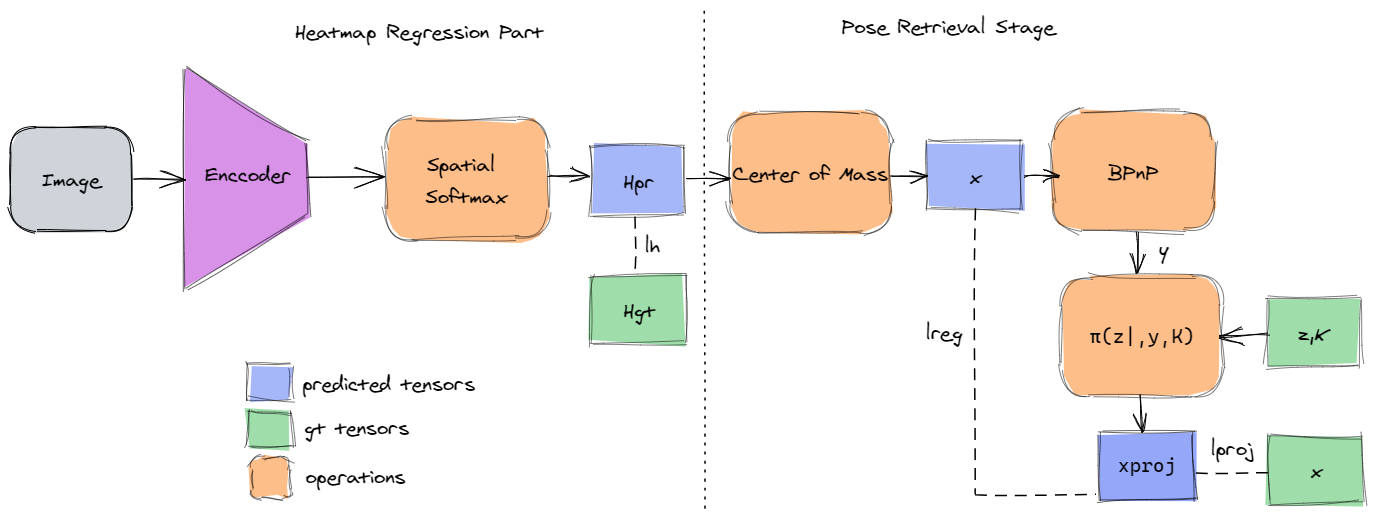
\includegraphics[scale=0.25]{../openreview/figures/method_5.png}
  \caption{Indirect object pose estimation approach consisting of the \textit{Heatmap Regression} part where HigherHRNet paper focuses on, and \textit{Pose Retrieval} part where BPnP focuses, alongside the supervision signals.}
\label{fig:methodology}
\end{figure*}


\subsection{Model descriptions}
\label{sec:models}
The following models were used as our backbone for regressing the heatmaps and the corresponding coordinate spatial distributions (the decoder part in Figure~\ref{fig:methodology}):
\begin{itemize}
    \item \textit{HRNet \cite{sun2019deep}} with feature maps of width 48 and 3 stages. 
    The 2nd, and 3rd, stages contain 1, 4 exchange blocks, respectively, and each exchange block contains 4 residual units.
    \item\textit{HigherHRNet \cite{cheng2020higherhrnet}} with feature maps of width 48 and 3 stages. 
    The 2nd, and 3rd, stages contain 1, 4 exchange blocks, respectively, and each exchange block contains 4 residual units.
    \item \textit{Stacked Hourglass \cite{newell2016stacked}} with depth 2 and feature maps of width 128
\end{itemize}

Following the heatmap predictions, we apply a decoding operation (\textit{i.e.}~center of mass specifically) in order to extract the keypoints from the heatmaps, which are later driven to the PnP algorithm for retrieving the 6D pose. %The heatmaps size was set to one fourth of the the input image size,which is 80x60 in our case.

In addition, we integrated the EPnP \cite{lepetit2009epnp} algorithm, using the available implementation in Pytorch3D \cite{ravi2020pytorch3d} instead of BPnP to assess whether other -- similar in concept -- implementations can verify the claim and quantify the differences between these approaches.
As a side-note, it should be mentioned that our models' configuration slightly differs from the ones described in the original works in order to comply with the working resolution of the dataset we used.

\subsection{Datasets}
\subsubsection{UAVA}

As aforementioned, our experiments were conducted on a dataset that allowed for the validation of both works simultaneously.
This also better helps in deducing whether the claims are reproducible as the context (task or dataset) can vary. 
We used the UAVA dataset\footnote{\url{https://vcl3d.github.io/UAVA/}} for object pose estimation. 
UAVA targets human-robot cooperative Unmanned Aerial Vehicle(UAV) applications and offers two different drone models, namely DJI M2ED\footnote{\url{https://www.dji.com/gr/mavic-2-enterprise}} and Ryze Tello\footnote{\url{https://www.ryzerobotics.com/tello}}.
%with the following statistics ... 
The UAVA dataset provides the 3D models of both drones accompanied by ground-truth annotations such as 3D bounding boxes, 6D pose, and at the same time multi-modal data.
More importantly, the difference in size between the two drone models allows for the validation of scale-invariant pose estimation.
%Mode details about the dataset creation, the training. validation and testing scripts can be found in the provided link.

%For each dataset include 1) relevant statistics such as the number of examples and label distributions, 2) details of train / dev / test splits, 3) an explanation of any preprocessing done, and 4) a link to download the data (if available).

\subsubsection{Preprocessing}
We processed the original dataset in order to keep only the samples where all the 2D keypoints are within the image, given that BPnP relies on softly approximating the coordinate, and that would fail in the case of out of field-of-view keypoints.
However, we should mention that we did not apply any other filtering (i.e. visibility of all the keypoints, boundary cases, etc.).

\subsection{Hyperparameters}
We train all the models for \textbf{44} epochs and select the best performing model for testing. 
We used the \textbf{Adam} optimizer with a learning rate of $1e-4$, betas of values $0.9$ and $0.999$ and no weight decay, and a seed value of 1989 for ensuring reproducibility.
Albeit, we experimented with different losses (\textit{i.e.}~KL, MSE) for $l_h$, we found that L1 loss works the best, offering the best results and faster convergence. 
This could be attributed to the different resolution of the heatmaps grid (in our case is lower) as well as the different configuration of the heatmap decoder model (we used 3 stages instead of 4). 
It is worth mentioning that we also tried a bigger heatmap resolution (\textit{e.g.}~$160 \times 120$) although we decided to conduct our final experiments in the lower resolution for two main reasons. 
First, most heatmaps regression decoders used in the literature make their prediction in the $\nicefrac{1}{4}$ of the original image, and second, this higher heatmap resolution would enforce us to further reduce the depth of the decoder model.
Specifically, for BPnP we set $\beta$ value to $1e-5$ after conducting a greedy heuristic search, with values ranging from $0.001$ to $1e-9$, as the proposed value for $\beta$ coefficient, did not work for our case. The selection of a non-appropriate $\beta$ coefficient value can lead to stability issues as noted in Section 5.2. 

%\subsection{Training procedure} 
%Following the approach proposed in the original paper \cite{chen2020end} we trained all models with $l_h$ loss only, for 30 epochs.After that, we trained the models for another 14 epochs by employing $l_m$ and $l_p$ losses. As the proposed value for $\beta$ coefficient did not work for our case, we set this value to $1e-5$ after conducting several manual experiments,with values ranging from 0.001 to 1e-9. We did not initialise the initial weights of our models and we use an Adam otpimizer with a learning rate of 1e-4 and betas [0.0,0.99], eps 1e-8 with no weight decay.
%More details for the exact configuration of each experiment is provided with the associated config file (TODO--add link?).
%Describe how the hyperparameter values were set. If there was a hyperparameter search done, be sure to include the range of hyperparameters searched over, the method used to search (e.g. manual search, random search, Bayesian optimization, etc.), and the best hyperparameters found. Include the number of total experiments (e.g. hyperparameter trials). You can also include all results from that search (not just the best-found results).

%ADD a table

\subsection{Experimental setup and code}
As mentioned above, we integrated the authors' code (BPnP) or our own reimplementations (HigherHRNet) in \cite{moai} which is a PyTorch framework for modular and reproducible workflows\footnote{\href{https://github.com/ai-in-motion/moai}{www.github.com/ai-in-motion/moai}}.
Each model is implemented in a configuration file that defines the different components (optimizer, datasets, model architecture, pre-/post-processing graphs, etc.) and logs all hyperparameters.
For each experiment we report the standard metrics below:
%Therefore, in order to fit moai's requirements, we adapted the code provided from both authors, and provide results in various well-established pose metrics described below.% such as the normalised positional error (NPE), angular distance in rads (AD), position and rotation accuracy (ACC),6d pose (ADD) and projection (Proj).

\textbf{NPE}: is the magnitude (L2-norm) of difference between the ground-truth and estimated position vectors from the origin of the camera reference frame to that of the drone body frame, normalised with  ground-truth vector.

\textbf{AD}: is the angular distance between the predicted, rotation matrix, and ground-truth,or in other words, the magnitude of the rotation that aligns the drone body frame with the camera reference frame.

\textbf{ACC}: considers an estimated pose to be correct if its rotation error is within \textbf{k$^{\circ}$} and the translation error is below \textbf{k cm}.

\textbf{ADD}: is the average distance metric to compute the averaged distance between points transformed using the estimated pose and the ground truth pose. 
Eventually, a pose estimation is considered to be correct if the computed average distance is within \textbf{k\%} of the model diagonal.

\textbf{Proj}: is the mean distance between 2D keypoints projected with the estimated pose and those projected with ground truth pose. 
An estimated pose is considered correct if this distance is within a threshold \textbf{k}.

%Include a description of how the experiments were set up that's clear enough a reader could replicate the setup. 
%Include a description of the specific measure used to evaluate the experiments (e.g. accuracy, precision@K, BLEU score, etc.). 
%Provide a link to your code.

\subsection{Computational requirements}
Table~\ref{tab:durations} showcases the total duration of each experiment (with a 24 batch size) as well as some other useful statistics such as the mean duration time for a forward pass, a backward pass, an optimizer step, as well as the total test duration with batch size 1. 
It is clear, that the introduction of the differentiable PnP modules in the training procedure increases the total training time significantly, as the backward and step operation require more time.
We ran our experiments on a machine with the specifications presented in Table~\ref{Hardware components}.
% Please add the following required packages to your document preamble:
% \usepackage{multirow}
% \usepackage[table,xcdraw]{xcolor}
% If you use beamer only pass "xcolor=table" option, i.e. \documentclass[xcolor=table]{beamer}
\begin{table}[hbt!]
\caption{Time statistics for each experiment. \textcolor{Red}{Red} and \textcolor{Orange}{orange} colors indicate the two (worst, and second worst respectively) most time-consuming experiment per drone model.}
\label{tab:durations}
\resizebox{\textwidth}{!}{\begin{tabular}{c|l|ccccc}
\hline
Drone &  & \textbf{\begin{tabular}[c]{@{}c@{}}Total \\ Training \\ Duration (hrs)\end{tabular}} & \textbf{\begin{tabular}[c]{@{}c@{}}Mean \\ Model Fwd \\ Duration(s)\end{tabular}} & \textbf{\begin{tabular}[c]{@{}c@{}}Mean \\ Model Bwd \\ Duration(s)\end{tabular}} & \textbf{\begin{tabular}[c]{@{}c@{}}Mean \\ Optimizer \\ Step (s)\end{tabular}} & \textbf{\begin{tabular}[c]{@{}c@{}}Total \\ Test \\ Duration (min)\end{tabular}} \\ \hline
 & $l_m$ & {\cellcolor{Orange} 14.14} & 0.13 & {\cellcolor{Red} 2.73} & {\cellcolor{Red} 2.89} & 23.75 \\
 & $l_p$ & {\cellcolor{Orange} 14.13} & 0.13 & {\cellcolor{Red} 2.73} & {\cellcolor{Red} 2.90} & 19.30 \\
 & EPnP & {\cellcolor{Red} 17.33} & 0.19 & {\cellcolor{Orange} 1.49} & {\cellcolor{Orange} 1.74} & 24.37 \\
 & HRNet & 11.19 & 0.06 & \textbf{0.003} & \textbf{0.21} & 19.87 \\
 & Hourglass & \textbf{6.99} & 0.14 & 0.019 & 0.22 & 15.85 \\
\multirow{-6}{*}{\textit{M2ED}} & HigherHRNet & 10.54 & 0.11 & 0.033 & 0.36 & 23.63 \\ \hline
\multicolumn{1}{l|}{} &  $l_m$ & {\cellcolor{Orange} 20.78} & 0.13 & {\cellcolor{Orange} 2.72} & {\cellcolor{Orange} 2.9} & 23.82 \\
\multicolumn{1}{l|}{} & $l_p$ & {\cellcolor{Orange} 20.38} & 0.13 & {\cellcolor{Orange} 2.68} & {\cellcolor{Orange} 2.85} & 19.95 \\
\multicolumn{1}{l|}{} & EPnP & {\cellcolor{Red} 21.80} & 0.28 & {\cellcolor{Red} 3.80} & {\cellcolor{Red} 4.14} & 19.13 \\
\multicolumn{1}{l|}{} & HRNet & \textbf{9.69} & 0.13 & 0.029 & 0.38 & 19.88 \\
\multicolumn{1}{l|}{} & Hourglass & 10.13 & 0.14 & \textbf{0.020} & \textbf{0.22} & 15.62 \\
\multicolumn{1}{l|}{\multirow{-6}{*}{\textit{Tello}}} & HigherHRNet & 16.10 & 0.14 & 0.032 & 0.4 & 20.50 \\ \hline
\end{tabular}}
\end{table}
%\begin{wraptable}{l}{7.1cm}
\begin{table}[hbt!]
\centering
\caption{Hardware Components}
\label{Hardware components}
\begin{tabular}{l|l}
\hline
\textit{OS}      & Windows Microsoft Pro (x64)   \\
\textit{Storage} & 3TB Toshiba HDD               \\
\textit{CPU}     & Intel i9-7900X (4.30 GHz)     \\
\textit{GPU}     & GeForce RTX 2080 Ti (12 GB)   \\
\textit{RAM}     & 4 x 16 GB Kingston (2666 MHz)
\end{tabular}
\end{table}
%\end{wraptable}
%Include a description of the hardware used, such as the GPU or CPU the experiments were run on. 
%For each model, include a measure of the average runtime (e.g. average time to predict labels for a given validation set with a particular batch size).
%For each experiment, include the total computational requirements (e.g. the total GPU hours spent).
%(Note: you'll likely have to record this as you run your experiments, so it's better to think about it ahead of time). Generally, consider the perspective of a reader who wants to use the approach described in the paper --- list what they would find useful.

\section{Results}
\label{sec:results}
Our results support the claims presented by both authors in \cite{chen2020end} and \cite{cheng2020higherhrnet} respectively. 
As is demonstrated in Table~\ref{tab:results_bpnp}, the model trained with $l_p$ achieved better results in most of the metrics for both drone models. 
Similarly, Table~\ref{tab:results_higher} indicates that HigherHRNet yields better results for the small-scale drone in most of the metrics, although its performance for the bigger M2ED drone is worse compared to the standard HRNet model.
%Start with a high-level overview of your results. Do your results support the main claims of the original paper? Keep this section as factual and precise as possible, reserve your judgement and discussion points for the next "Discussion" section. 
%\section{Results}
\label{sec:results}

Given a fixed training FLOP budget, \textit{RigL} surpasses existing dynamic sparse training methods over a range of target sparsities, on both CIFAR-10 and 100 (Sections \ref{cifar-10-results}, \ref{cifar-100-results}). By training longer, \textit{RigL} matches or marginally outperforms iterative pruning. However, unlike pruning, its FLOP consumption is constant throughout. This a prime reason for using sparse networks, and makes training larger networks feasible. Finally, as evaluated on CIFAR-10, the original authors' choice of hyper-parameters are close to optimal for multiple target sparsities and initialization schemes (Section \ref{hyperparameter-tuning}).

\jdcomment{Start with a high-level overview of your results. \sout{Does your work support the claims you listed in section 2?} Keep this section as factual and precise as possible, reserve your judgement and discussion points for the next "Discussion" section. 

\textbf{Results reproducing original paper}
For each experiment, say 1) which claim in Section~\ref{sec:claims} it supports, and 2) if it successfully reproduced the associated experiment in the original paper. \sout{how it relates to one of the claims and explain what your result is.} 
For example, an experiment training and evaluating a model on a dataset may support a claim that that model outperforms some baseline.
Logically group related results into sections.} 

\subsection{WideResNet-22 on CIFAR-10}\label{cifar-10-results}

\begin{table}[t]
    \captionsetup{aboveskip=\tableaboveskip,belowskip=\tablebelowskip}
    \caption{\textbf{WideResNet-22-2 on CIFAR10}, tabulated for two density $(1-s)$ values. We group methods by their FLOP requirement and in each group, we mark the best accuracy in bold. Similar to \citet{rigl}, we assume that algorithms utilize sparsity during training. All results are obtained by methods implemented in our unified codebase.}
    \label{tab:cifar10-main-results}
    \centering
    
    \begin{tabular}{ c cc cc }
    \toprule
    \multirow{3}{*}{\textbf{Method}}& 
    \multicolumn{2}{c}{$\mathbf{1 - s=0.1}$} & \multicolumn{2}{c}{$\mathbf{1 - s=0.2}$} \\
    \cmidrule(lr){2-3} \cmidrule(lr){4-5}
    {} & 
    \makecell{Accuracy $\uparrow$ \\ (Test)}  & \makecell{FLOPs $\downarrow$  \\ (Train, Test)} &
    \makecell{Accuracy $\uparrow$ \\ (Test)}  & \makecell{FLOPs $\downarrow$  \\ (Train, Test)} \\
    \midrule
    Small Dense & 
    {89.0 $\pm$ 0.35} & {0.11x, 0.11x} & 
    {91.0 $\pm$ 0.07} & {0.20x, 0.20x} \\
    
    Static & 
    {89.1 $\pm$ 0.17} & {0.10x, 0.10x} & 
    {91.2 $\pm$ 0.16} & {0.20x,0.20x} \\

    SET &
    {91.3 $\pm$ 0.47} & {0.10x, 0.10x} & 
    \textbf{92.7 $\pm$ 0.28} & {0.20x, 0.20x} \\
    
    \textbf{RigL} &
    \textbf{91.7 $\pm$ 0.18} & {0.10x, 0.10x} &
    {92.6 $\pm$ 0.10} & {0.20x, 0.20x} \\
    \midrule
    
    SET (ERK)&
    {92.2 $\pm$ 0.04} & {0.17x, 0.17x} &
    {92.9 $\pm$ 0.16} & {0.35x, 0.35x} \\
    
    \textbf{RigL (ERK)} &
    \textbf{92.4 $\pm$ 0.06} & {0.17x, 0.17x} &
    \textbf{93.1 $\pm$ 0.09} & {0.35x, 0.35x} \\
    \midrule
    {Static\textsubscript{$2 \times$}} &
    {89.15 $\pm$ 0.17} & {0.20x, 0.10x} &
    {91.2 $\pm$ 0.16} & {0.40x, 0.20x} \\
    
    Lottery & 
    {90.4 $\pm$ 0.09} & {0.45x, 0.13x} & 
    {92.0 $\pm$ 0.31} & {0.68x,0.27x} \\
    
    {SET\textsubscript{$2 \times$}} &
    {83.3 $\pm$ 15.33} & {0.20x, 0.10x} &
    {93.0 $\pm$ 0.22} & {0.41x, 0.20x} \\
    
    SNFS & 
    {92.4 $\pm$ 0.43} & {0.51x, 0.27x} & 
    {92.7 $\pm$ 0.20} & {0.66x, 0.49x} \\ 
    
    SNFS (ERK)& 
    {92.2 $\pm$ 0.2} & {0.52x, 0.28x} & 
    {92.8 $\pm$ 0.07} & {0.66x, 0.49x} \\
    
    {SNFS\textsubscript{$2 \times$}} &
    {92.3 $\pm$ 0.33} & {1.02x, 0.27x} &
    {93.2 $\pm$ 0.14} & {1.32x, 0.98x} \\
    
    {RigL\textsubscript{$2 \times$}} &
    {92.3 $\pm$ 0.25} & {0.20x, 0.10x} &
    {93.0 $\pm$ 0.21} & {0.41x, 0.20x} \\
    
    % {RigL\textsubscript{$3 \times$}} &
    % {92.5 $\pm$ 0.11} & {0.30x, 0.10x} &
    % {93.2 $\pm$ 0.20} & {0.61x, 0.20x} \\
    
    {Pruning} & 
    {92.6 $\pm$ 0.08} & {0.32x,0.13x} & 
    {93.2 $\pm$ 0.27} & {0.41x,0.27x} \\ 
    
    \textbf{RigL\textsubscript{$2 \times$} (ERK)} &
    \textbf{92.7 $\pm$ 0.37} & {0.34x, 0.17x} &
    \textbf{93.3 $\pm$ 0.09} & {0.70x, 0.35x} \\
    \midrule
    
    \textbf{Dense Baseline} &
    \textbf{93.4 $\pm$ 0.07} & {9.45e8, 3.15e8} &
    \textbf{-} & {-} \\
    \bottomrule
    
    \end{tabular}
\end{table}
   
Results on the CIFAR-10 dataset are provided in Table \ref{tab:cifar10-main-results}. Tabulated metrics are averaged across 3 random seeds and reported with their standard deviation. All sparse networks use random initialization, unless indicated otherwise.

While SET improves over the performance of static sparse networks and small-dense networks, methods utilizing gradient information (SNFS, \textit{RigL}) obtain better test accuracies. SNFS can outperform \textit{RigL}, but requires a much larger training budget, since it (a) requires dense gradients at each training step, (b) redistributes layer-wise sparsity during mask updates. For all sparse methods, excluding SNFS, using ERK initialization improves performance, but with increased FLOP consumption. We calculate theoretical FLOP requirements in a manner similar to \citet{rigl} (exact details in the supplementary material). 

Figure \ref{fig:cifar10-main-results} contains test accuracies of select methods across two additional sparsity values: ($0.5, 0.95$). At lower sparsities (higher densities), \textit{RigL} matches the performance of the dense baseline. Performance further improves by training for longer durations. Particularly, training \textit{RigL} (ERK) twice as long at 90\% sparsity exceeds the performance of iterative pruning while requiring similar theoretical FLOPs. This validates the original authors' claim that \textit{RigL} (a sparse-to-sparse training method) outperforms pruning (a dense-to-sparse training method). 

\begin{figure}[!t]
    \centering
    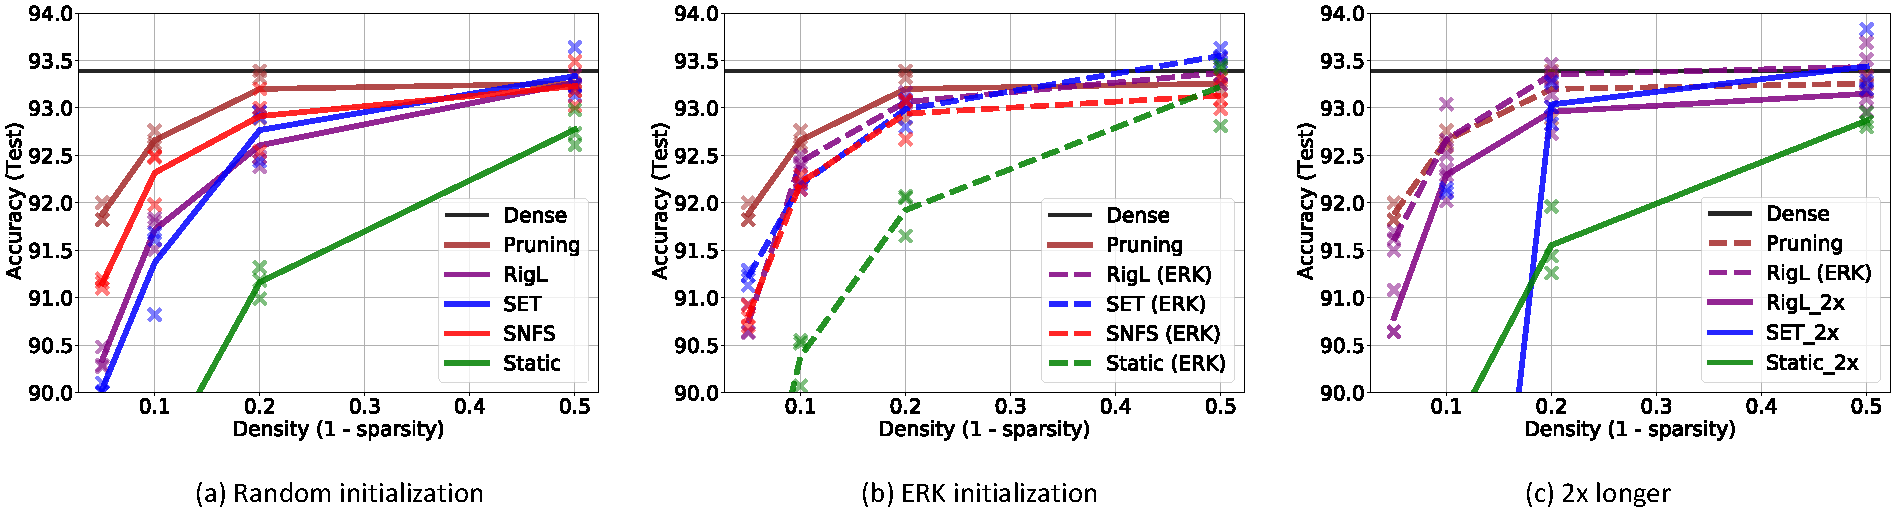
\includegraphics[width=1\textwidth]{../openreview/figs/cifar10_main.pdf}
    \captionsetup{aboveskip=\figureaboveskip,belowskip=\figurebelowskip}
    \caption{\textbf{Test Accuracy vs Sparsity on CIFAR-10,} plotted for Random initialization \textbf{(left)}, ERK initialization \textbf{(center)}, and for training $2\times$ longer \textbf{(right)}. Owing to random growth, SET can be unstable when training for longer durations with higher sparsities. Overall, \textit{RigL}\textsubscript{$2 \times$} (ERK) achieves highest test accuracy.}
    \label{fig:cifar10-main-results}
\end{figure}
\subsection{ResNet-50 on CIFAR100}\label{cifar-100-results}

\begin{tabularx}{\textwidth}[hb]{*{2}{>{\centering\arraybackslash}X}}
    \centering
    \captionsetup{labelformat=andfigure,width=1.1\linewidth,aboveskip=7pt,belowskip=0pt}
    \captionlistentry[figure]{entry for figure}
    \label{fig:cifar100-main-results}
    
    \captionof{table}{\textbf{Benchmarking sparse ResNet-50s on CIFAR-100,} tabulated by performance and cost \textbf{(below)}, and plotted across densities \textbf{(right)}. In each group below, \textit{RigL} outperforms or matches existing sparse-to-sparse and dense-to-sparse methods. Notably, \textit{RigL}\textsubscript{$3\times$} at 90\% sparsity and \textit{RigL}\textsubscript{$2\times$} at 80\% sparsity surpass iterative pruning with similar FLOP consumption. \textit{RigL}\textsubscript{$2\times$} (ERK) further improves performance but requires a larger training budget. }
    \resizebox{1.15\linewidth}{!}{%
\begin{tabular}{ c cc cc }
\toprule
\multirow{3}{*}{\textbf{Method}}& 
\multicolumn{2}{c}{$\mathbf{1 - s=0.1}$} & \multicolumn{2}{c}{$\mathbf{1 - s=0.2}$} \\
\cmidrule(lr){2-3} \cmidrule(lr){4-5}
{} & 
\makecell{Accuracy $\uparrow$ \\ (Test)}  & \makecell{FLOPs $\downarrow$  \\ (Train, Test)} &
\makecell{Accuracy $\uparrow$ \\ (Test)}  & \makecell{FLOPs $\downarrow$  \\ (Train, Test)} \\
\midrule
Static & 
{69.7 $\pm$ 0.42} & {0.10x, 0.10x} & 
{72.3 $\pm$ 0.30} & {0.20x,0.20x} \\

Small Dense & 
{70.8 $\pm$ 0.22} & {0.11x, 0.11x} & 
{72.6$\pm$ 0.93} & {0.20x, 0.20x} \\

SET &
{71.4 $\pm$ 0.35} & {0.10x, 0.10x} & 
{73.4 $\pm$ 0.45} & {0.20x, 0.20x} \\

\textbf{RigL} &
\textbf{71.8 $\pm$ 0.33} & {0.10x, 0.10x} &
\textbf{73.5 $\pm$ 0.04} & {0.20x, 0.20x} \\
\midrule

Static (ERK) & 
{71.5 $\pm$ 0.18} & {0.22x, 0.22x} & 
{73.2 $\pm$ 0.39} & {0.38x, 0.38x} \\

SET (ERK)&
{72.3 $\pm$ 0.39} & {0.22x, 0.22x} &
\textbf{73.5 $\pm$ 0.25} & {0.38x, 0.38x} \\

\textbf{RigL (ERK)} &
\textbf{72.6 $\pm$ 0.37} & {0.23x, 0.22x} &
{73.4 $\pm$ 0.15} & {0.38x, 0.38x} \\
\midrule

SNFS & 
{72.3 $\pm$ 0.20} & {0.58x, 0.37x} & 
{73.9 $\pm$ 0.20} & {0.70x, 0.55x} \\ 

SNFS (ERK)& 
{73.0 $\pm$ 0.33} & {0.59x, 0.38x} & 
{73.9 $\pm$ 0.27} & {0.69x, 0.54x} \\

{Pruning} & 
{73.1 $\pm$ 0.32} & {0.36x,0.11x} & 
{73.8 $\pm$ 0.23} & {0.45x,0.25x} \\ 

{RigL\textsubscript{$2 \times$}} &
{73.1 $\pm$ 0.71} & {0.20x, 0.10x} &
{74.0 $\pm$ 0.24} & {0.41x, 0.20x} \\

{Lottery} &
{73.6 $\pm$ 0.32} & {0.62x,0.11x} & 
{74.2 $\pm$ 0.41} & {0.81x,0.25x} \\

\textbf{RigL\textsubscript{$3 \times$}} &
\textbf{73.7 $\pm$ 0.16} & {0.30x, 0.10x} &
{74.2 $\pm$ 0.23} & {0.61x, 0.20x} \\

\textbf{RigL\textsubscript{$2 \times$} (ERK)} &
{73.6 $\pm$ 0.05} & {0.46x, 0.22x} &
\textbf{74.4 $\pm$ 0.10} & {0.76x, 0.38x} \\

\midrule

\textbf{Dense Baseline} &
\textbf{74.7 $\pm$ 0.38} & {7.77e9, 2.59e9} &
\textbf{-} & {-} \\
\bottomrule

\end{tabular}%
}

    \label{tab:cifar100-main-results}  
&
    \centering
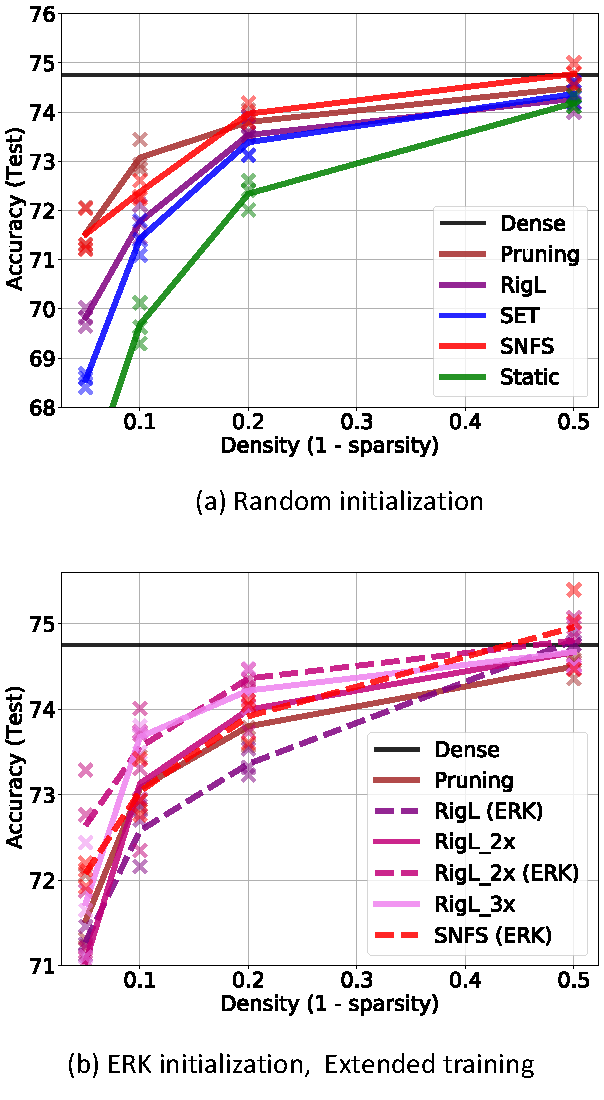
\includegraphics[width=0.66\linewidth,valign=t]{../openreview/figs/cifar100_main.pdf}
\end{tabularx}

We see similar trends when training sparse variants of ResNet-50 on the CIFAR-100 dataset (Table \ref{tab:cifar100-main-results}, metrics reported as in Section \ref{cifar-10-results}). We also include a comparison against sparse networks trained with the Lottery Ticket Hypothesis (\citet{frankle2018lottery}) in Table \ref{tab:cifar100-main-results}---we obtain tickets with a commensurate performance for sparsities lower than 80\%. Finally, the choice of initialization scheme affects the performance and FLOP consumption by a greater extent than the method used itself, with the exception of SNFS (groups 1 and 2 in Table \ref{tab:cifar100-main-results}). 


\subsection{Hyperparameter Tuning}\label{hyperparameter-tuning}

\begin{table}[th]
    \captionsetup{aboveskip=\tableaboveskip,belowskip=\tablebelowskip}
    \caption{\textbf{Reference vs Optimal $(\alpha, \Delta T)$ on CIFAR-10.} Optimal hyperparameters are obtained by tuning with a TPE sampler in Optuna. The difference between the reference and optimal performance is small, indicating that there is not a significant benefit in tuning $(\alpha, \Delta T)$ individually for each initialization and sparsity configuration.}
    \label{tab:effect-alpha-deltaT}
    \centering
    
    \begin{tabular}{ c c  cc  cc}
    \toprule
    \multirow{3}{*}{\textbf{Initialization}} & \textbf{Density} & 
    \multicolumn{2}{c}{\textbf{Reference}} & \multicolumn{2}{c}{\textbf{Optimal}} \\
    \cmidrule(lr){2-2} \cmidrule(lr){3-4} \cmidrule(lr){5-6}
    {} & {$(1-s)$} & 
    {$(\alpha, \Delta T)$} & \makecell{Accuracy $\uparrow$ \\ (Test)} & 
    {$(\alpha, \Delta T)$} & \makecell{Accuracy $\uparrow$ \\ (Test)} \\
    \midrule
    
    Random & 0.1 & 
    {0.3, 100} & {91.7 $\pm$ 0.18} &  
    {0.197, 50} & \textbf{91.8 $\pm$ 0.17} \\
    
    Random & 0.2 & 
    {0.3, 100} & {92.6 $\pm$ 0.10} &  
    {0.448, 150} & \textbf{92.8 $\pm$ 0.16} \\
    
    Random & 0.5 & 
    {0.3, 100} & \textbf{93.3 $\pm$ 0.07} &  
    {0.459, 550} & \textbf{93.3 $\pm$ 0.18} \\
    \midrule
    
    ERK & 0.1 & 
    {0.3, 100} & \textbf{92.4 $\pm$ 0.06} &  
    {0.416, 200} & \textbf{92.4 $\pm$ 0.23} \\
    
    ERK & 0.2 & 
    {0.3, 100} & \textbf{93.1 $\pm$ 0.09} &  
    {0.381, 950} & \textbf{93.1 $\pm$ 0.21} \\
    
    ERK & 0.5 & 
    {0.3, 100} & {93.4 $\pm$ 0.14} &  
    {0.287, 500} & \textbf{93.8 $\pm$ 0.06} \\
    \hline

    \end{tabular}
    
    \label{tab:replication_verify}
\end{table}

\subsubsection{$(\alpha, \Delta T)$ vs Sparsities} To understand the impact of the two additional hyperparameters included in \textit{RigL}, we use a Tree of Parzen Estimator (TPE sampler, \citet{TPE_Bergstra}) via Optuna to tune $(\alpha, \Delta T)$. We do this for sparsities $(1 - s) \in \{0.1,0.2,0.5\}$, and a fixed learning rate of $0.1$. Additionally, we set the sampling domain for $\alpha$ and $\Delta T$ as $[0.1,0.6]$ and $\{50,100, 150,...,1000\}$ respectively. We use 15 trials for each sparsity value, with our objective function as the validation accuracy averaged across 3 random seeds.

\begin{figure}[!b]
    \centering
    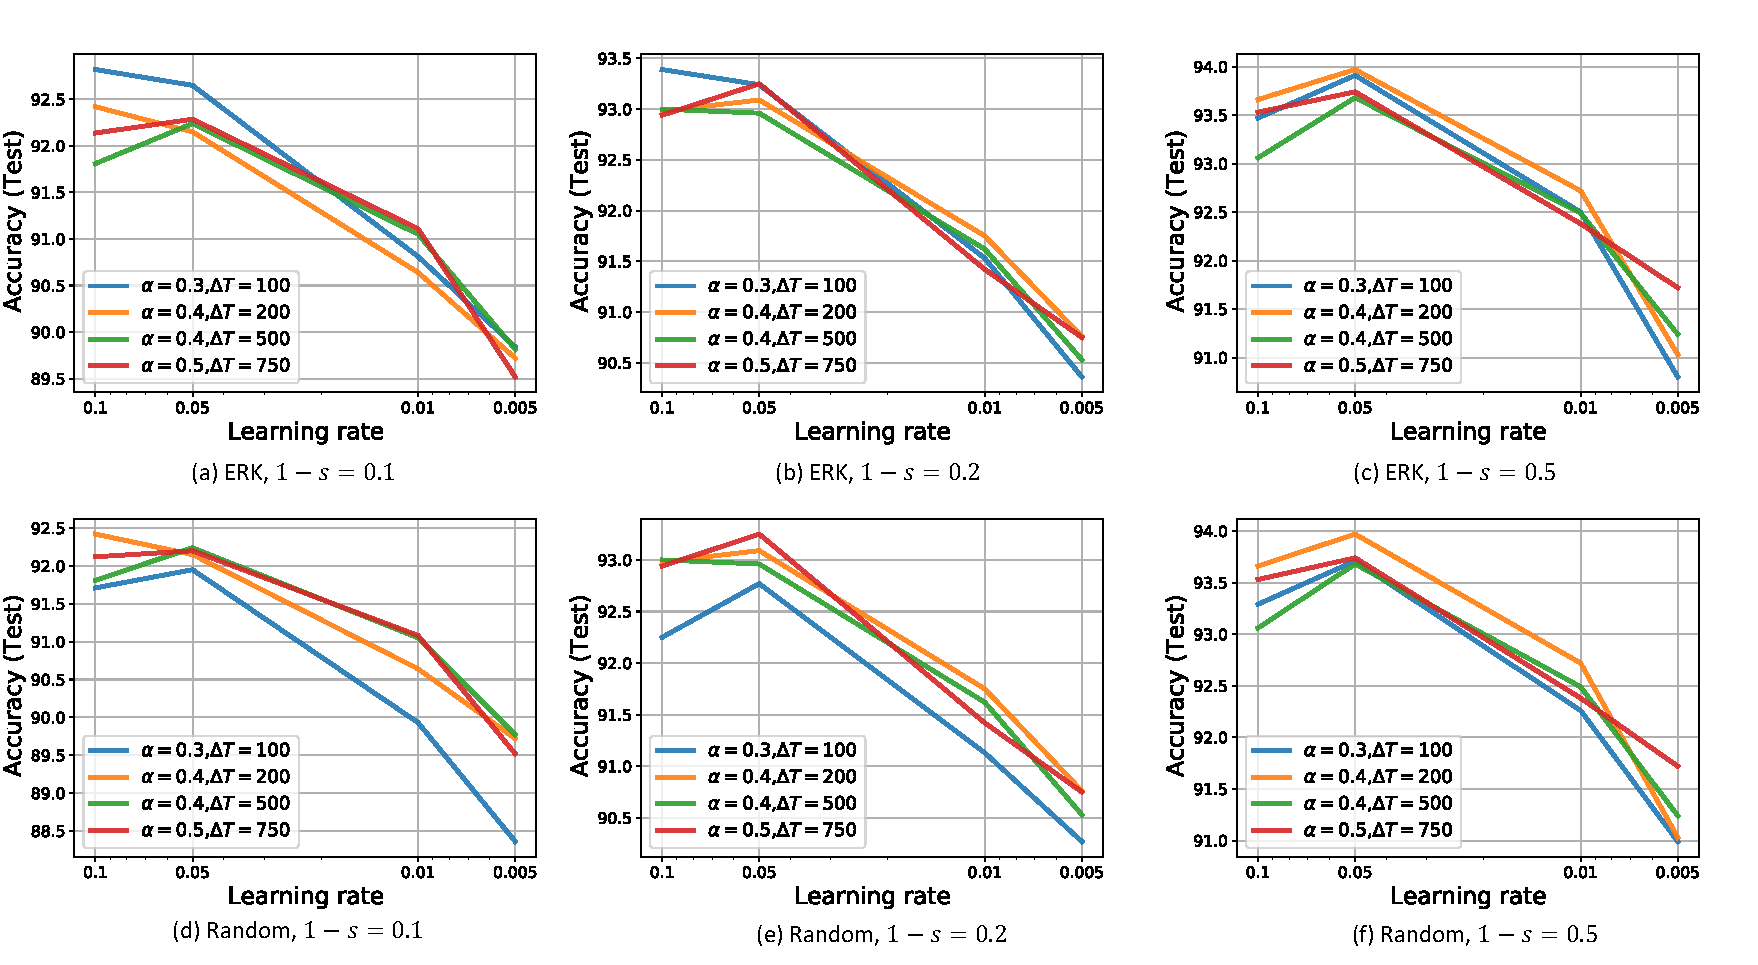
\includegraphics[width=\textwidth]{../openreview/figs/lr_sweep.pdf}
    \captionsetup{aboveskip=\figureaboveskip,belowskip=\figurebelowskip}
    \caption{\textbf{Learning Rate vs Sparsity on CIFAR-10.} Runs using a learning rate $> 0.1$ do not converge and are not plotted here. There is little benefit in tuning the learning rate for each sparsity, and $0.1, 0.05$ are good choices overall.}
    \label{fig:lr-sweep}
\end{figure}

Table \ref{tab:effect-alpha-deltaT} shows the test accuracies of tuned hyperparameters. While the reference hyperparameters (original authors, $\alpha=0.3, \Delta T=100$) differ from the obtained optimal hyperparameters, the difference in performance is marginal, especially for ERK initialization. This in agreement with the original paper, which finds $\alpha \in \{0.3, 0.5\}, \Delta T = 100$ to be suitable choices. We include contour plots detailing the hyperparameter trial space in the supplementary material.

\subsubsection{Learning Rate vs Sparsities} We further examine if the final performance improves by tuning the learning rate ($\eta$) individually for each sparsity-initialization pair. We employ a grid search over $\eta \in \{0.1,0.05,0.01,0.005\}$ and $(\alpha, \Delta T) \in \{(0.3, 100), (0.4,200), (0.4, 500), (0.5, 750)\}$. As seen in Figure \ref{fig:lr-sweep}, $\eta = 0.1$ and $\eta = 0.05$ are close to optimal values for a wide range of sparsities and initializations. Since these learning rates also correspond to good choices for the Dense baseline, one can employ similar values when training with \textit{RigL}.




\subsection{Results reproducing original papers}
%For each experiment, say 1) which claim in Section~\ref{sec:claims} it supports, and 2) if it successfully reproduced the associated experiment in the original paper. 
%For example, an experiment training and evaluating a model on a dataset may support a claim that that model outperforms some baseline.
%Logically group related results into sections. 
\subsubsection{BPnP}
With these experiments we show that the addition of a differentiable PnP module improves the performance in object pose estimation task.
We provide qualitative results in Figure~\ref{fig:qualitativeboth}. 
It is worth highlighting that training with $l_p$ does not restrict the shape of the distribution the way that it is constrained when relying on heatmap supervision (\textit{i.e.}~Gaussian distribution approximation).
Instead, the model freely localizes the keypoints, which results in more focused predictions. 
This is illustrated in Figure~\ref{fig:qualitativehtmps} where qualitative results display the heatmaps on top of the color images. 
% Please add the following required packages to your document preamble:
% \usepackage{multirow}
% \usepackage[table,xcdraw]{xcolor}
% If you use beamer only pass "xcolor=table" option, i.e. \documentclass[xcolor=table]{beamer}
\begin{table}[hbt!]
\centering
\caption{BPnP results on the UAVA dataset. We trained all models for 44 epochs and select the best among them for inference. Light \textcolor{SeaGreen}{green} with \textbf{bold} and light \textcolor{Cerulean}{blue} indicate the best and second best performers.}
\label{tab:results_bpnp}
\resizebox{\textwidth}{!}{\begin{tabular}{l|l|llllllll}
\hline
Drone &  & \textbf{NPE$\downarrow$} & \textbf{AD$\downarrow$} & \textbf{ACC2$\uparrow$} & \textbf{ACC5$\uparrow$} & \textbf{ADD2$\uparrow$} & \textbf{ADD5$\uparrow$} & \textbf{Proj2$\uparrow$} & \textbf{Proj5$\uparrow$} \\ \hline
 & $l_m$ & 0.014 & 0.027 & \cellcolor{MyLightBlue}92.13 & \cellcolor{MyLightBlue}98.07 & \cellcolor{MyLightBlue}81.31 & \cellcolor{MyLightBlue}93.34 & \cellcolor{MyLightGreen}\textbf{99.45} & \cellcolor{MyLightGreen}\textbf{99.58} \\
 & $l_p$ & \cellcolor{MyLightBlue}0.012 & \cellcolor{MyLightBlue}0.026 & \cellcolor{MyLightGreen}\textbf{95.20} & \cellcolor{MyLightGreen}\textbf{98.36} & \cellcolor{MyLightGreen}\textbf{90.29} & \cellcolor{MyLightGreen}\textbf{96.81} & \cellcolor{MyLightBlue}98.05 & 99.14 \\
\multirow{-3}{*}{\textit{M2ED}} & $l_h$ & \cellcolor{MyLightGreen}\textbf{0.011} & \cellcolor{MyLightGreen}\textbf{0.020} & 90.75 & 98.04 & 80.52 & 91.37 & 97.56 & \cellcolor{MyLightBlue}99.49 \\ \hline
 & $l_m$ & \cellcolor{MyLightBlue}0.071 & \cellcolor{MyLightGreen}\textbf{0.189} & \cellcolor{MyLightBlue}43.38 & \cellcolor{MyLightBlue}82.11 & 14.88 & 41.47 & \cellcolor{MyLightGreen}93.97 & \cellcolor{MyLightGreen}\textbf{96.08} \\
 & $l_p$ & \cellcolor{MyLightGreen}\textbf{0.063} & \cellcolor{MyLightBlue}0.223 & \cellcolor{MyLightGreen}\textbf{55.31} & \cellcolor{MyLightGreen}\textbf{85.34} & \cellcolor{MyLightGreen}\textbf{20.04} & \cellcolor{MyLightGreen}\textbf{50.53} & \cellcolor{MyLightBlue}\textbf{93.19} & \cellcolor{MyLightBlue}94.49 \\
\multirow{-3}{*}{\textit{Tello}} & $l_h$ & 0.091 & 0.252 & 36.36 & 74.99 & \cellcolor{MyLightBlue}18.27 & \cellcolor{MyLightBlue}43.31 & 89.25 & 94.00 \\ \hline
\end{tabular}}
\end{table}
\begin{figure*}[hbt!]
  \centering
  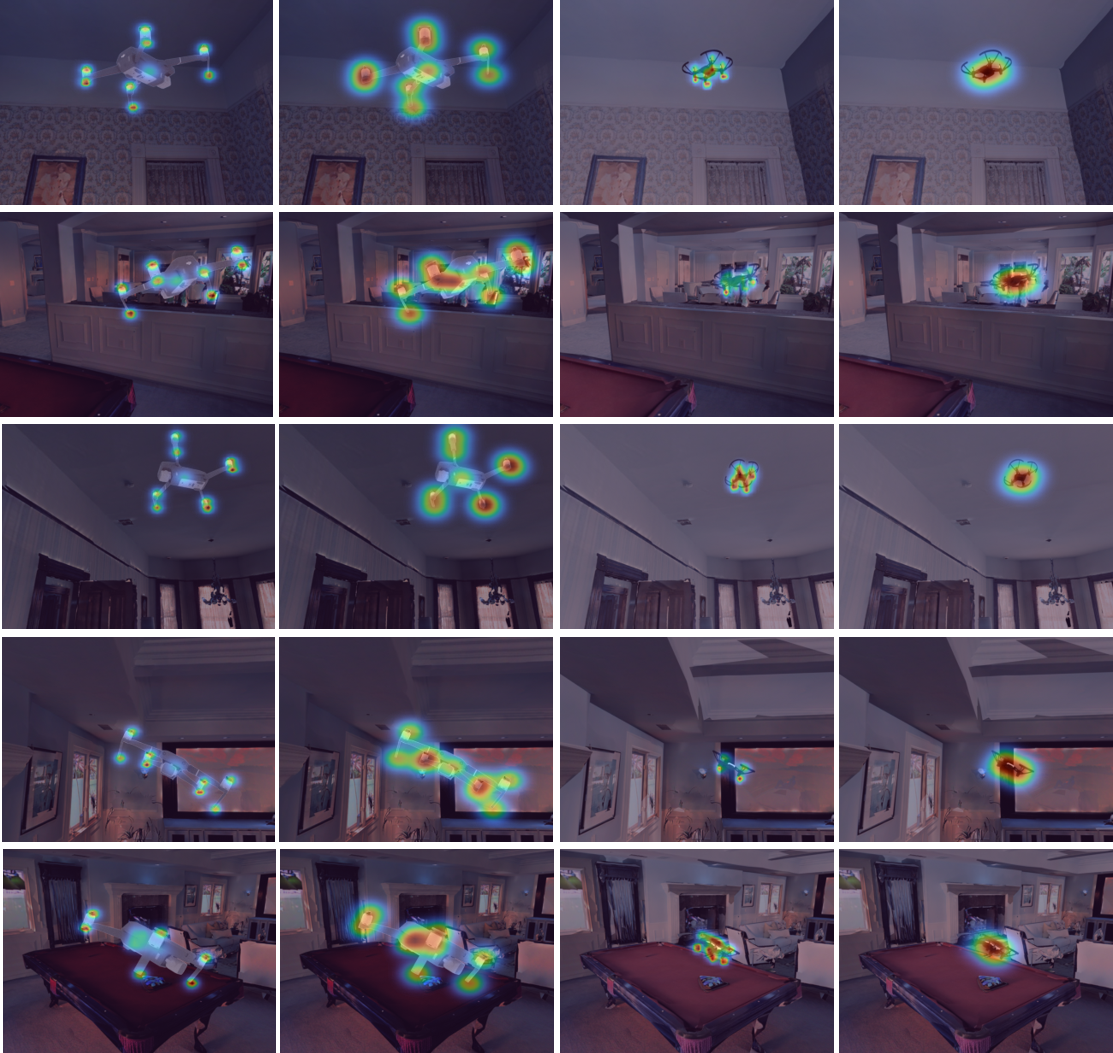
\includegraphics[scale=0.70]{../openreview/figures/qualitativeheatmaps.png}
  \caption{Qualitative heatmap results on random samples from the test-set. 
  The first \textbf{two} columns depicts the M2ED drone while the last \textbf{two} the Tello drone; with heatmaps predicted by models trained with $l_p$ and $l_h$ respectively.
  Evidently, heatmaps by the $l_h$ model (\textbf{second and fourth columns} tend to keep the 2D Gaussian shape distribution, while the $l_p$ ones (\textbf{first and third columns}) freely approximate the $(x,y)$ position enforced by the regularizer term($l_{reg}$) of the $l_p$ loss, eventually allowing for more distinguishable 2D keypoints estimations.}
\label{fig:qualitativehtmps}
\end{figure*}
\subsubsection{HigherHRNet}
These experiments showcase that the addition of the aggregation module improves the keypoint localization performance when targeting smaller-scale objects. 
Specifically, the HigherHRNet architecture gives better results in most of the metrics for the small form drone (Tello). 
On the other hand though, this is not the case for the larger drone, where the HigherHRNet performance is slightly worse than the standard HRNet's one. 
% Please add the following required packages to your document preamble:
% \usepackage{multirow}
% \usepackage[table,xcdraw]{xcolor}
% If you use beamer only pass "xcolor=table" option, i.e. \documentclass[xcolor=table]{beamer}
\begin{table}[hbt!]
\centering
\caption{HigherHRNet results on the UAVA dataset. We trained all models for 44 epochs and select the best among them for inference. Light \textcolor{SeaGreen}{green} with \textbf{bold} and light \textcolor{Cerulean}{blue} indicate the best and second best performers.}
\label{tab:results_higher}
\resizebox{\textwidth}{!}{\begin{tabular}{l|l|llllllll}
\hline
drone &  & \textbf{NPE$\downarrow$} & \textbf{AD$\downarrow$} & \textbf{ACC2$\uparrow$} & \textbf{ACC5$\uparrow$} & \textbf{ADD2$\uparrow$} & \textbf{ADD5$\uparrow$} & \textbf{Proj2$\uparrow$} & \textbf{Proj5$\uparrow$} \\ \hline
 & Hourglass & 0.015 & 0.028 & 89.43 & 96.94 & 78.20 & 90.42 & 96.56 & 99.02 \\
 & HRNet & 
 \cellcolor{MyLightGreen}\textbf{0.011} & \cellcolor{MyLightGreen}\textbf{0.020} & \cellcolor{MyLightGreen}\textbf{90.75} & \cellcolor{MyLightGreen}\textbf{98.04} & \cellcolor{MyLightGreen}\textbf{80.52} & \cellcolor{MyLightGreen}\textbf{91.37} & \cellcolor{MyLightGreen}\textbf{97.56} & \cellcolor{MyLightGreen}\textbf{99.49} \\
\multirow{-3}{*}{\textit{M2ED}} & HigherHRNet & \cellcolor{MyLightGreen}\textbf{0.011} & \cellcolor{MyLightGreen}\textbf{0.020} & \cellcolor{MyLightBlue}89.92 & \cellcolor{MyLightBlue}97.75 & \cellcolor{MyLightBlue}79.58 & \cellcolor{MyLightBlue}90.99 & \cellcolor{MyLightBlue}97.50 & \cellcolor{MyLightBlue}99.44 \\ \hline
 & Hourglass & \cellcolor{MyLightBlue}0.094 & \cellcolor{MyLightGreen}\textbf{0.214} & 32.19 & \cellcolor{MyLightBlue}75.47 & 14.76 & 38.26 & \cellcolor{MyLightGreen}\textbf{92.23} & \cellcolor{MyLightGreen}\textbf{96.25} \\
 & HRNet & \cellcolor{MyLightGreen}\textbf{0.091} & \cellcolor{MyLightBlue}0.252 & \cellcolor{MyLightBlue}36.36 & 74.99 & \cellcolor{MyLightBlue}18.27 & \cellcolor{MyLightBlue}43.31 & 89.25 & \cellcolor{MyLightBlue}94.00 \\
\multirow{-3}{*}{\textit{Tello}} & HigherHRNet & 0.095 & 0.264 & \cellcolor{MyLightGreen}\textbf{42.98} & \cellcolor{MyLightGreen}\textbf{75.69} & \cellcolor{MyLightGreen}\textbf{20.19} & \cellcolor{MyLightGreen}\textbf{46.69} & \cellcolor{MyLightBlue}89.54 & 93.63 \\ \hline
\end{tabular}}
\end{table}
\subsection{Results beyond the BPnP paper}
Apart from the experiments conducted by the authors in \cite{chen2020end} we provide additional to further support the main claims. 
Particularly, we compared BPnP versus an alternative differentiable PnP algorithm (\textit{i.e.}~EPnP) and the results are demonstrated in Table~\ref{tab:bpnpvsepnp}. 
We also provide extra experiments of a BPnP implementation in which the calculation of the higher-order derivatives is ignored from the coefficient's graph as presented in Table~\ref{tab:results_FasterBPnP}.
%Often papers don't include enough information to fully specify their experiments, so some additional experimentation may be necessary. For example, it might be the case that batch size was not specified, and so different batch sizes need to be evaluated to reproduce the original results. Include the results of any additional experiments here. Note: this won't be necessary for all reproductions.
\subsubsection{BPnP vs EPnP}
For this experiment we utilised the same backbone (\textit{i.e.}~HRNet) but we changed the BPnP module with the EPnP. 
We followed the exact same training procedure, hyperparameters, as well as the same loss $l_m$. 
Results are summarized in Table~\ref{tab:bpnpvsepnp}.
It is evident that EPnP and BPnP offers comparable results in most of the metrics. 
% Please add the following required packages to your document preamble:
% \usepackage{multirow}
% \usepackage[table,xcdraw]{xcolor}
% If you use beamer only pass "xcolor=table" option, i.e. \documentclass[xcolor=table]{beamer}
\begin{table}[hbt!]
\centering
\caption{BPnP vs EPnP. Following the same approach we trained the decoder part only with $l_h$ for 30 epochs and then continue with $l_m$ for 14 epochs. Light \textcolor{SeaGreen}{green} with \textbf{bold} indicates the best performer.}
\label{tab:bpnpvsepnp}
\resizebox{\textwidth}{!}{\begin{tabular}{l|l|llllllll}
\hline
Drone &  & \textbf{NPE$\downarrow$} & \textbf{AD$\downarrow$} & \textbf{ACC2$\uparrow$} & \textbf{ACC5$\uparrow$} & \textbf{ADD2$\uparrow$} & \textbf{ADD5$\uparrow$} & \textbf{Proj2$\uparrow$} & \textbf{Proj5$\uparrow$} \\ \hline
 & BPnP & \cellcolor{MyLightGreen}\textbf{0.014} & \cellcolor{MyLightGreen}\textbf{0.027} & 92.13 & 98.07 & \cellcolor{MyLightGreen}\textbf{81.31} & 93.34 & 99.45 & 99.58 \\
\multirow{-2}{*}{\textit{M2ED}} & EPnP & \cellcolor{MyLightGreen}\textbf{0.014} & \cellcolor{MyLightGreen}\textbf{0.027} & \cellcolor{MyLightGreen}\textbf{92.89} & \cellcolor{MyLightGreen}\textbf{98.19} & 80.50 & \cellcolor{MyLightGreen}\textbf{93.64} & \cellcolor{MyLightGreen}\textbf{99.52} & \cellcolor{MyLightGreen}\textbf{99.61} \\ \hline
 & BPnP & \cellcolor{MyLightGreen}\textbf{0.071} & \cellcolor{MyLightGreen}\textbf{0.189} & 43.38 & \cellcolor{MyLightGreen}\textbf{82.11} & 14.88 & 41.47 & \cellcolor{MyLightGreen}\textbf{93.97} & 96.08 \\
\multirow{-2}{*}{\textit{Tello}} & EPnP & 0.074 & 0.192 & \cellcolor{MyLightGreen}\textbf{46.77} & 81.64 & \cellcolor{MyLightGreen}\textbf{21.07} & \cellcolor{MyLightGreen}\textbf{49.59} & 93.77 & \cellcolor{MyLightGreen}\textbf{96.13} \\ \hline
\end{tabular}}
\end{table}
\subsubsection{BPnP$_{faster}$}
Authors in \cite{chen2020end} provided an alternative method for calculating the gradients through the PnP layer, which essentially is the same method as the original, although ignoring the higher-order derivatives from the coefficients graph.
Therefore, we provide results using this faster BPnP method in Table~\ref{tab:results_FasterBPnP}, comparing the two different versions, as well as their training times in Table~\ref{tab:FasterBPnP_duration}. 
It seems that the original version outmatches the faster one, albeit there is no significant performance drop. 
On the other hand, Table~\ref{tab:FasterBPnP_duration} indicates how the second implementation justifies its name. So, it is in users' fluency whether they need to sacrifice gradient accuracy and some performance drop in exchange for efficient training times.
% Please add the following required packages to your document preamble:
% \usepackage{multirow}
% \usepackage[table,xcdraw]{xcolor}
% If you use beamer only pass "xcolor=table" option, i.e. \documentclass[xcolor=table]{beamer}
\begin{table}[hbt!]
\centering
\caption{BPnP$_{faster}$ results on the UAVA dataset, following the exact training approach as original BPnP. Here we present results with models trained with $l_p$. Light \textcolor{SeaGreen}{green} with \textbf{bold} indicates the best performer. }
\label{tab:results_FasterBPnP}
\resizebox{\textwidth}{!}{\begin{tabular}{l|l|llllllll}
\hline
Drone &  & \textbf{NPE$\downarrow$} & \textbf{AD$\downarrow$} & \textbf{ACC2$\uparrow$} & \textbf{ACC5$\uparrow$} & \textbf{ADD2$\uparrow$} & \textbf{ADD5$\uparrow$} & \textbf{Proj2$\uparrow$} & \textbf{Proj5$\uparrow$} \\ \hline
 & BPnP$_{faster}$ & 0.013 & 0.029 & 94.79 & 98.06 & 89.38 & 96.66 & 97.83 & 98.98 \\
\multirow{-2}{*}{\textit{M2ED}} & BPnP & \cellcolor{MyLightGreen}\textbf{0.012} & 
\cellcolor{MyLightGreen}\textbf{0.026} & \cellcolor{MyLightGreen}\textbf{95.20} & \cellcolor{MyLightGreen}\textbf{98.36} & \cellcolor{MyLightGreen}\textbf{90.29} & \cellcolor{MyLightGreen}\textbf{96.81} & \cellcolor{MyLightGreen}\textbf{98.05} & \cellcolor{MyLightGreen}\textbf{99.14} \\ \hline
 & BPnP$_{faster}$ & \cellcolor{MyLightGreen}\textbf{0.055} & \cellcolor{MyLightGreen}\textbf{0.167} & \cellcolor{MyLightGreen}\textbf{55.42} & \cellcolor{MyLightGreen}\textbf{87.03} & \cellcolor{MyLightGreen}\textbf{26.43} & \cellcolor{MyLightGreen}\textbf{58.99} & \cellcolor{MyLightGreen}\textbf{94.91} & \cellcolor{MyLightGreen}\textbf{96.12} \\
\multirow{-2}{*}{\textit{Tello}} & BPnP & 0.063 & 0.223 & 55.31 & 85.34 & 20.04 & 50.53 & 93.19 & 94.49 \\ \hline
\end{tabular}}
\end{table}
% Please add the following required packages to your document preamble:
% \usepackage{multirow}
% \usepackage[table,xcdraw]{xcolor}
% If you use beamer only pass "xcolor=table" option, i.e. \documentclass[xcolor=table]{beamer}
\begin{table}[hbt!]
%\centering
\caption{BPnP$_{faster}$ time statistics. Light \textcolor{SeaGreen}{green} with \textbf{bold} indicates quicker performance.}
\label{tab:FasterBPnP_duration}
\resizebox{\textwidth}{!}{\begin{tabular}{c|l|ccccc}
\hline
Drone &  & \textbf{\begin{tabular}[c]{@{}c@{}}Total \\ Training \\ Duration (hrs)\end{tabular}} & \textbf{\begin{tabular}[c]{@{}c@{}}Mean \\ Model Fwd \\ Duration(s)\end{tabular}} & \textbf{\begin{tabular}[c]{@{}c@{}}Mean \\ Model Bwd \\ Duration(s)\end{tabular}} & \textbf{\begin{tabular}[c]{@{}c@{}}Mean \\ Optimizer \\ Step (s)\end{tabular}} & \textbf{\begin{tabular}[c]{@{}c@{}}Total \\ Test \\ Duration (min)\end{tabular}} \\ \hline
 & \textit{\begin{tabular}[c]{@{}l@{}}BPnP$_{faster}$\end{tabular}} & {\cellcolor{MyLightGreen} \textbf{6.80}} & 0.089 & {\cellcolor{MyLightGreen} \textbf{0.53}} & {\cellcolor{MyLightGreen} \textbf{0.66}} & 17.15 \\
\multirow{-2}{*}{\textit{M2ED}} & BPnP & { 14.13} & 0.13 & { 2.73} & { 2.90} & 19.30 \\ \cline{1-1}
\multicolumn{1}{l|}{} & \textit{\begin{tabular}[c]{@{}l@{}}BPnP$_{faster}$\end{tabular}} & {\cellcolor{MyLightGreen} \textbf{10.39}} & 0.09 & {\cellcolor{MyLightGreen} \textbf{0.54}} & {\cellcolor{MyLightGreen} \textbf{0.69}} & 18.85 \\
\multicolumn{1}{l|}{\multirow{-2}{*}{\textit{Tello}}} & BPnP & { 20.38} & 0.13 & { 2.68} & { 2.85} & 19.95 \\ 
%\cline{1-1}
\hline
\end{tabular}}
\end{table}
\section{Discussion}
\begin{figure*}[hbt!]
  \centering
  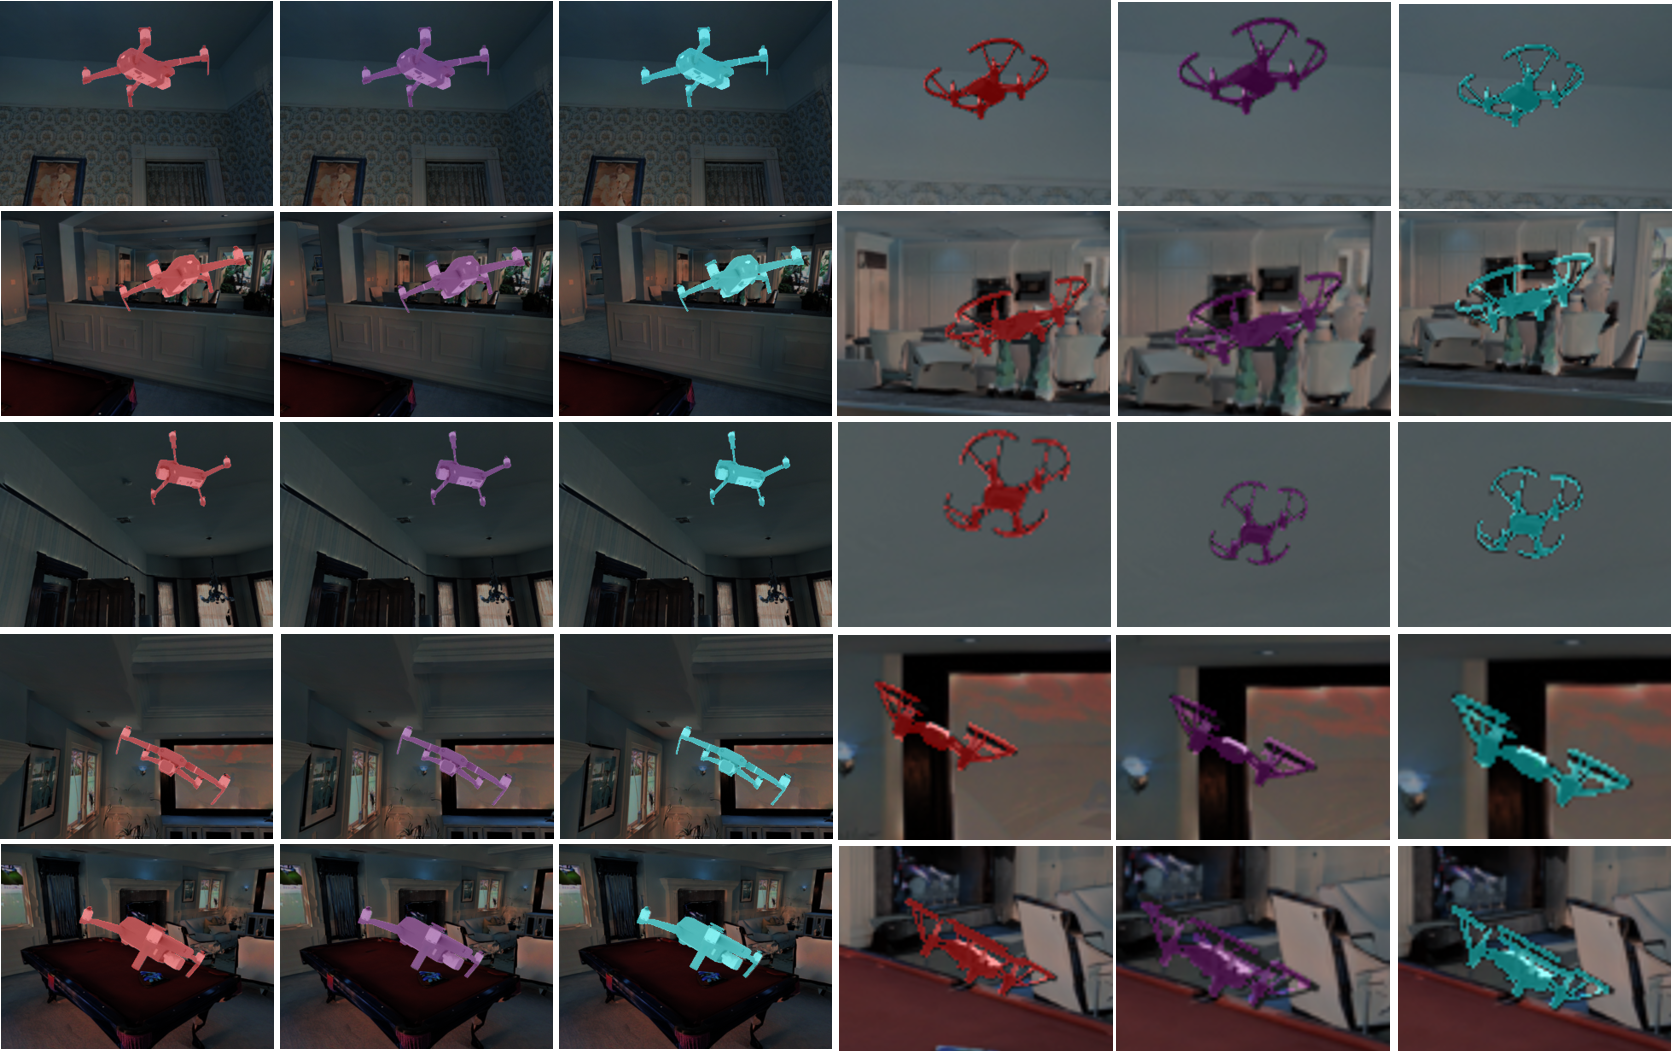
\includegraphics[scale=0.45]{../openreview/figures/qualitativeboth_2.png}
  \caption{Qualitative results on random samples from the UAVA dataset from three different models. The \emph{\color{red}\textbf{red}} mask indicates predictions by $l_p$ trained model, \emph{\color{purple}\textbf{purple}} by $l_m$ and finally \emph{\color{cyan}\textbf{cyan}} by HRNet. 
  The drone masks are rendered by employing the predicted pose(i.e. output of the BPnP) and then blended with the original color image. 
  The first \textbf{three} columns depicts M2ED drone model while the rest \textbf{three} the Tello drone. 
  The Tello samples are cropped and zoomed-in due to its small form factor.}
\label{fig:qualitativeboth}
\end{figure*}
%Give your judgement on if your experimental results support the claims of the paper. Discuss the strengths and weaknesses of your approach - perhaps you didn't have time to run all the experiments, or perhaps you did additional experiments that further strengthened the claims in the paper.
After conducting several experiments on the UAVA dataset, the central claims of \cite{chen2020end} and \cite{cheng2020higherhrnet} stand true; as they both outperform other methods. 
Particularly, for validating BPnP we conducted the same experiments as the original paper, and further, we compare it with another differentiable PnP method (\textit{i.e.}~EPnP). 
The inclusion of 2D-3D geometry constraints through differentiable geometric optimization, improves the performance.
Extending the experiments of the original paper, we compare another implementation of the BPnP module which ignores the high order derivatives from the coefficient graph. 
This module achieves comparable results as its counterpart apart it is much faster. It is worth noting, that both BPnP, and EPnP are quite time-consuming as demonstrated in Table~\ref{tab:durations}. 
Finally, we study the performance of the HigherHRNet \cite{chen2020end} in a very challenging small scale object. Indeed, the performance of the proposed heatmap aggregation module achieves better results when compared with other well-established methods.
\subsection{What was easy}
Implementing most of the code was straightforward as authors of both papers provide source code. 
GitHub issues were another source of retrieving information, clarifying parts of the papers when needed. 
Additionally, both of the original papers are quite complete, well-written making it easy to follow.
%Give your judgement of what was easy to reproduce. Perhaps the author's code is clearly written and easy to run, so it was easy to verify the majority of original claims. Or, the explanation in the paper was really easy to follow and put into code. 

%Be careful not to give sweeping generalizations. Something that is easy for you might be difficult to others. Put what was easy in context and explain why it was easy (e.g. code had extensive API documentation and a lot of examples that matched experiments in papers). 

\subsection{What was difficult}

%List part of the reproduction study that took more time than you anticipated or you felt were difficult. 

%Be careful to put your discussion in context. For example, don't say "the maths was difficult to follow", say "the math requires advanced knowledge of calculus to follow". 

Our major difficulty was related to finding the appropriate value for balancing the terms of mixture loss $l_m$, aka the $\beta$ value.
Even though, authors in \cite{chen2020end} provided the value that they used for their experiments this did not work for us, as this is a case specific parameter.
It is worth noting that a non-appropriate selection of the balancing term can lead to convergence issues and negative results. 
Even though, not related with the code of both of the papers, we feel that it would be constitutive to mention that we faced the same difficulties when trying to incorporate EPnP in our workflow.

\subsection{Communication with original authors}
%Document the extent of (or lack of) communication with the original authors. To make sure the reproducibility report is a fair assessment of the original research we recommend getting in touch with the original authors. You can ask authors specific questions, or if you don't have any questions you can send them the full report to get their feedback before it gets published. 

Authors of \cite{chen2020end} did not specify the configuration of the used network in the pose estimation task, nor the hyperparameters. 
Thus, we contacted them through GitHub where they provided a detailed answer, available now to the research community.
We did not contact HigherHRNet authors \cite{cheng2020higherhrnet} as the online implementations and the text and figures in their paper were a good enough guide to understand and implement it.

\section*{Acknowledgements}
This research has been supported by the European Commission funded program \href{https://www.faster-project.eu/}{FASTER}, under H2020 Grant Agreement 833507.

%\bibliographystyle{unsrt}  
%\bibliography{refs}
%\bibliography{bibliography}